\section{Framework and Tools}
In this section, we gradually develop the framework. First, we give a high-level overview of the system. Second, we decide what data source to use initially and describe how to use the data. Third, we present the method of choice to perform initial data filtering. Fourth, we agree on which data storage and ingestion to use. Fifth, we provide a methodology to group the data. Sixth, we decide how users will interact with the obtained results. Last, we select the visualisation tools to be used.
%In this section, we evaluate what data sources are useful. Additionally, we discuss several methods and tools that can be helpful in storing and ingesting data. Furthermore, we describe numerous methods to filter and classify textual data. Then, we elaborate on different methods to perform queries with. We conclude with an overview of the available visualisation tools that can be used for displaying the results of the analysis.
\section{High-level Overview}
The figure below represents a high-level overview of the system. The most important inputs, outputs and steps in system the are displayed. A more in-depth explanation of the different stages of the process can be found in the following sections.

\begin{figure}[ht]
\centering
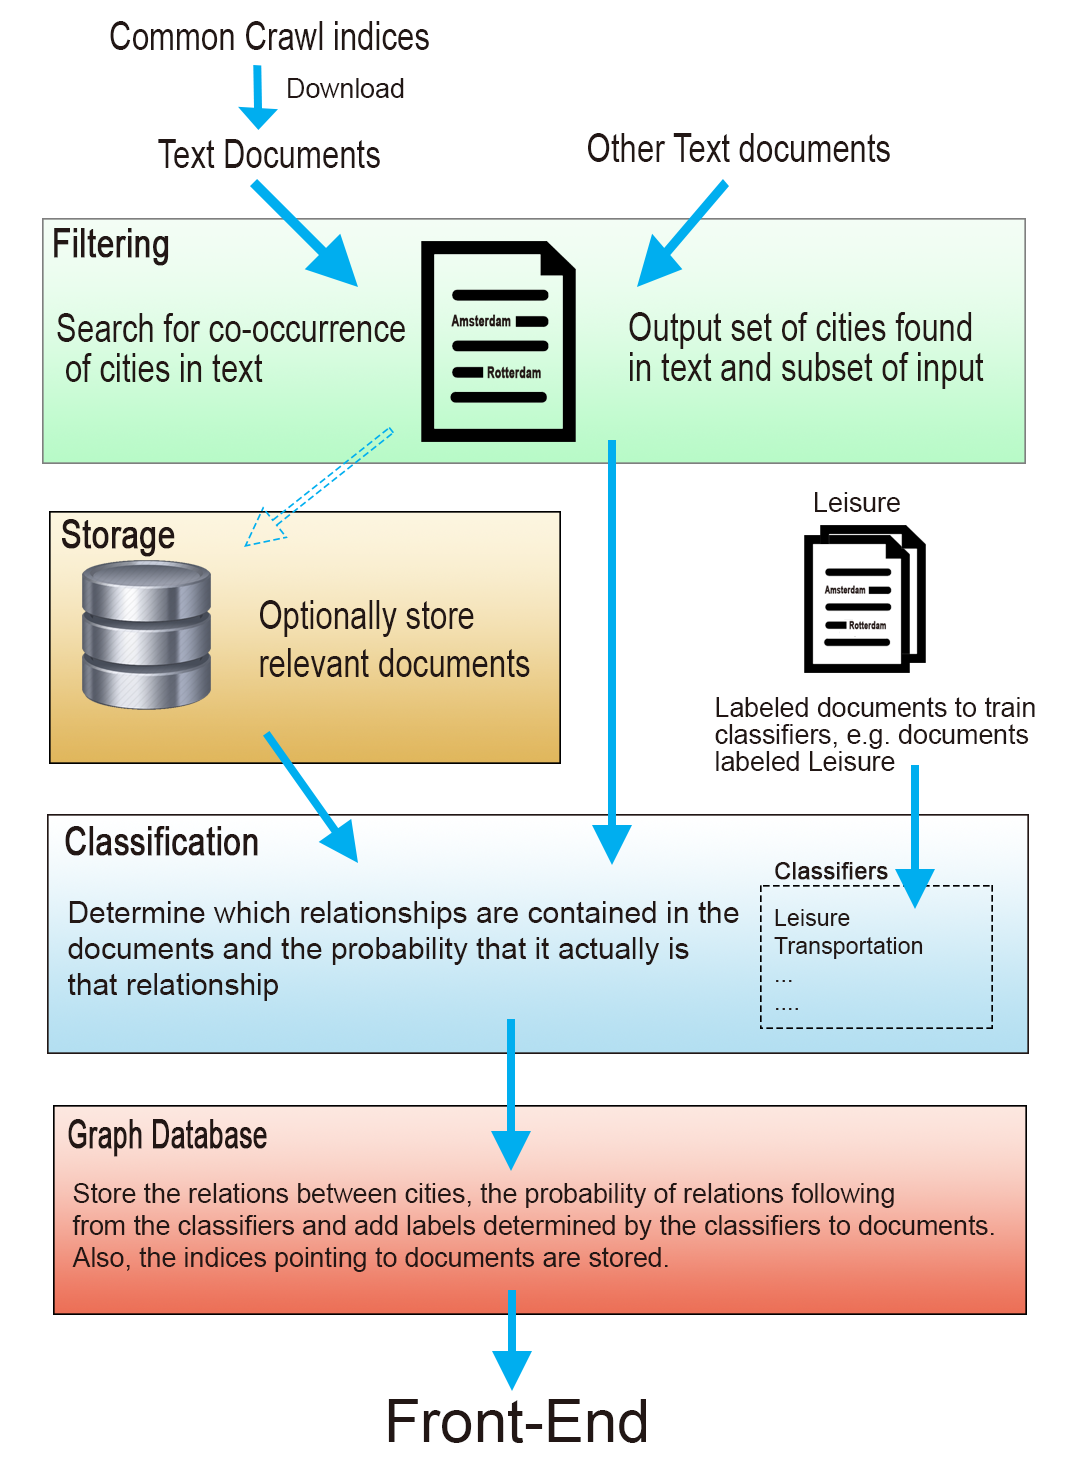
\includegraphics[width=0.8\textwidth]{System-overview-3}
\caption{High-level overview of the system}
\label{fig:overview}
\end{figure}
\subsection{Gathering the Data}
As explained in subsection \ref{sec:design-goals}, data sources should be plugable. An initial corpus of documents is needed to base the project, which we will decide on in this subsection. 

\subsubsection{Common Crawl} \label{sec:commoncrawl}
Common Crawl \cite{commoncrawl} is a freely accessible corpus of pages across the web, updated and released on a monthly basis. Many researchers have used the data for various purposes
\cite{smith2013dirt, muhleisen2012web, singh2012wikilinks}.
Since the project requires analysis on a very large set of documents, the corpus is a very suitable candidate for us to work with. \\

The data from Common Crawl comes in three formats\footnote{\url{https://gist.github.com/Smerity/e750f0ef0ab9aa366558}}: 
\begin{description}
\item[\textbf{WARC}] This is the default and most verbose format. It stores the HTTP-response, information about the request and meta-data on the crawl process itself. The content is stored as HTML-content.
\item[\textbf{WAT}] Files of this type contain meta-data, such as link addresses, about the WARC-records. This meta-data is computed for each of the three types of records (meta-data, request, and response). The textual content of the page is not present in this format.
\item[\textbf{WET}] This format only contains extracted plain text. No HTML-tags are present in this text. For our purposes, this is the most useful format.
\end{description}

Common Crawl stores these pages in the following way: each archive is split into many segments, with each segment representing a directory. Every directory contains a document listing file and a folder for each file format (WARC, WAT and WET), which in turn contains the compressed pages belonging to the segment. To be able to efficiently get a single page, Common Crawl indexes the segments to directly map URLs to document locations using an offset and length which can be found using the Common Crawl index\footnote{\url{http://index.commoncrawl.org}}. Since WAT- and WET-files can be generated from WARC-files, they only provide such indices for WARC-files. If no file index is provided with a data request, an aggregated compressed file of all files of the requested format is returned.

For extracting data from Common Crawl, many open-source libraries are available. Common Crawl's official website refers to \texttt{cdx-index-client}\footnote{\url{https://github.com/ikreymer/cdx-index-client}} as a command line interface to their data indices. It allows for, among others, specifying which data set to use, supports multiple output formats (plain text, gzip or JSON) and can run in parallel. Since this library only retrieves the file indices, we need another way to actually retrieve the pages pointed to. However, there is a problem with this: we are only interested in WET-files, but Common Crawl does not have WET-files indexed. We would therefore have to collect the WARC-files and convert them to WET-files ourselves, requiring us to parse HTML for every document we are interested in.

A simple query on the latest index using the online interface\footnote{\url{http://index.commoncrawl.org/CC-MAIN-2017-13-index?url=*.nl&output=json&showNumPages=true}} yields 1676 pages. Pages in this sense are listings of 15000 indices, so there are roughly 25 million entries in total. It is very important to note that searching for a top level domain like \texttt{.nl} only includes the first page of every matching domain. To get all pages, additional queries for each site with more than one page are to be performed.


\subsubsection{Other Data Sources}\label{sec:delpher}
Besides Common Crawl, there are a plethora of other sources that might contain valuable information. The most notable is the Dutch royal library, Delpher\footnote{\url{http://delpher.nl}}. It contains millions of Dutch digitalised newspapers, books and magazines from the fifteenth century up until about 1995. Because of this, it is a useful resource for historical research. Additionally, Statistics Netherlands\footnote{\url{https://www.cbs.nl/en-gb}} is the governmental organisation collecting statistical data about the Netherlands and comes with an API, making most of their data publicly accessible. The NOW Corpus\footnote{\url{http://corpus.byu.edu/now/}} collects newspaper and magazine articles through Google News and provides several tools to perform queries on this data. It can also be downloaded. 

Due to time and resource constraints, we have chosen to exclude these from the project. Of course, in future versions, other data sources could be included.



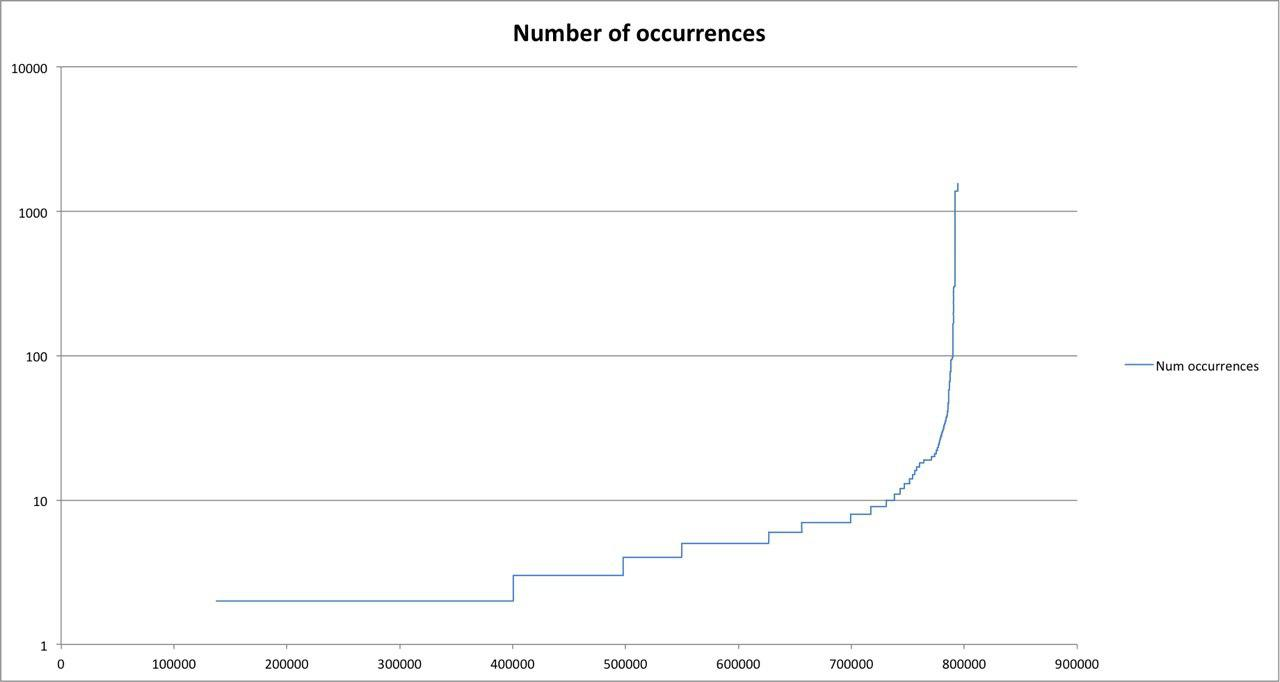
\includegraphics[width=\textwidth]{occurences_per_page}
% \todo{add info:}

% Piet Bep, [16.06.17 11:55]
% num 20
% 773665
% num 30
% 7510
% num 40
% 4020
% num 50
% 979

% Piet Bep, [16.06.17 11:55]
% bovenstaande is aantal documenten met minder dan 20 occurrences, tussen 20 en 30, tussen 30 en 40, en tussen 40 en 50
\subsection{Filtering Documents}
Because not all data from information sources such as Common Crawl is relevant to find relationships between cities, the data needs to be filtered. One way to do this, is to only select the data that mentions at least two different cities. Because the data is plain text, we need a way to scan through the text and determine if the text indeed has a co-occurrence of two different cities.
Making use of the comparative analysis of Rasool et al. \cite{rasool2012string}, we chose the Aho-Corasick algorithm \cite{Aho-Corasick}, which is a multi-pattern exact string matching algorithm and is the driver of widely used tools such as \texttt{grep} \cite{kernighan1984unix}. The algorithm creates a finite state machine, where strings to match are final states. Since we are looking for the co-occurrence of cities, using a multi-pattern string matching algorithm is preferred over a plain string matching algorithm. This is especially well illustrated by table \ref{tab:bm-matching} below. The benchmark was performed on a string of 1500 characters, with a million iterations. In the table, the average speed of matching is shown in seconds.

\begin{table}
\centering
\begin{tabular}{ |c|c| } 
    \hline
    multi-pattern matching & 0.000049831339 \\
    plain string matching & 0 \\
    \hline
\end{tabular}
\caption{Benchmark of multi-string vs. plain string matching}
\label{tab:bm-matching}
\end{table}

Using the Aho-Corasick algorithm, a predefined list of cities can be matched against the text of a web page or document. If at least two cities from the list appear in the text, we mark it as a useful document.

The decision to use the Aho-Corasick algorithm is strengthened by the fact that a well documented and stable Python library exists, which implements the aforementioned algorithm. This library is called \texttt{pyahocorasick}\footnote{\url{https://pypi.python.org/pypi/pyahocorasick/}} and is a fast and memory efficient implementation of the Aho-Corasick algorithm.

We make a selection of documents without storing the documents first, because storing all documents is not feasible due to storage constraints. For the .nl web pages only would need about 250 GB of storage and to store all available documents around 250 TB of storage would be needed. As we do not have access to a fast and large data storage platform, we will not store everything first and then delete documents that were filtered out. However, to test if finding and storing relationships between cities is fast enough when the documents are actually stored on disk a random selection of 1 million documents will be downloaded. Processing the already stored documents could finish within one day\footnote{On a virtual server with 8GB RAM, 4 CPUs and 100GB of HDD storage.} whereas downloading all documents will most certainly take multiple days.

\subsection{Extracting Relations from Documents}
Now that a selection of relevant documents has been made, we can make an attempt to identify the relations between cities based on these documents. Since labelling every relevant document by hand is not feasible, an automated approach is desirable. 
One way to automate this process is by identifying intercity relations using machine learning. Machine learning algorithms can be roughly divided into two distinct groups: (1) supervised and (2) unsupervised algorithms. Supervised algorithms expect an input set and a corresponding output set, with which a model is trained to predict unseen instances of the problem. Unsupervised algorithms identify clusters of entities based on similarities in the feature set corresponding to said entity.
\replace{
Considering the fact that we have a strict time schedule of little over two months to develop the complete system, we decided to go with the supervised approach. 
The main reason for this choice is that the training and tweaking of supervised algorithms can be done faster compared to unsupervised algorithms. The main reason for this is that we do not need the complete data-set to start training a supervised model, while for the unsupervised case the complete set is needed.}{Lees dit nog effe goed, twee keer main reason en in feite geef je daarvoor al de main reason}

\subsubsection{Defining Classes}
Our choice of using classification has naturally lead to the need for categories we want to identify within the collected documents. Together with our clients, \replace{Dr. Evert Meijers and Antoine Peris}{beetje vreemd om die hier pas te into'en?}, we identified the following categories which are useful to identify from the collected documents:\\

\begin{enumerate}
    \item Collaboration
    \item Commuting
    \item Education
    \item Leisure
    \item Residential mobility
    \item Shopping
    \item Transportation
    \item Other
\end{enumerate}

These categories represent topics that are of interest for our clients. They relate to research that is being done by them and to relations that were deemed important in previous research on intercity relations. The category \textit{other} is there to make the classification exhaustive, i.e. relevant documents can always be labelled.

\subsubsection{Pre-processing}
For pre-processing the documents, there are a number of tools available. We used NLTK \cite{nlkt_stemming} for removing stopwords and regular expressions for removing unwanted characters. The HTML parsing/\todo{..} was done using BeautifulSoup.\todo{add ref}

\begin{description}
\item[\textbf{Stop words}]
Removing all common words (the, a, an etc) and symbols ('.', ',', '!', etc). For removing stopwords, we used a list from NLTK containing Dutch stopwords.

\item[\textbf{Unwanted characters}]
To strip unwanted characters we have defined a regular expression that identifies unwanted characters (punctuation marks, years, etc.) Matching characters are removed from the document. 

\item[\textbf{HTML}]
Since we are dealing with HTML pages which we are parsing to plain text documents, we need to strip the HTML so that only the plain text remains. Using BeautifulSoup we strip unwanted tags (script, style, link, etc.) and parse the rest of the page to plain text.
\end{description}

\subsubsection{Data-set}
Before we can start building up and training our model, we need to collect data that can be used as input for the model. To collect this data we have considered several options.\\

The first option is to query for documents from news(paper) sites. Since the documents are categorised by professionals, we may assume they will provide us with features that represent the categories associated with these documents well.
Unfortunately, the categories that we identified with our clients do not match typical newspaper categories, so this approach was not suitable for us.\\

Another approach is to use Google Custom Search to obtain results from Google, using the categories the client provided us with as keywords. The main disadvantage of this approach is lack of control over the files that get added into the data set and \todo{stukje over noise is zo'n typisch stukje waar claudolf de kriebels van krijgt. Hoe weet je dat er veel noise meekomt?} the large amount of noise produced by this method.\\

Finally, we decided to provide our clients with a "labelling interface". The labelling interface provides the user with a document from the set of collected documents. It allows the user to label these documents with zero or more categories, after which the document is assigned to the correct category. If no category is selected, the document is discarded from the training set. This way, we have total control of the documents that are added to the data set. The documents are labelled by experts in the field of the built environment so we may assume these documents will represent the labelled categories well. 

\subsubsection{Modelling}
When considering classification, there are a plethora of algorithms available. When choosing the right algorithm for a problem, several factors should be taken into account\cite{MLCheatSheet}. These are:
    \begin{description}
        \item[\textbf{Accuracy}] How well the algorithm separates the websites.
        \item[\textbf{Training Time}] How long it takes to train the algorithm.
        \item[\textbf{Linearity}] Linear regression assumes data trends follow a straight line. This is trade-off between accuracy and speed.
        \item[\textbf{Number of Parameters}] Adjustable parameters increase the flexibility of the algorithms. This is a trade-off between training time and accuracy.
        \item[\textbf{Number of Features}] A large number of features can make some algorithms slow. Especially text data (what we are using) has a high number of features.
        \item[\textbf{Special Cases}] Some learning algorithms make particular assumptions about the data or the results.
    \end{description}

Because of the fact that we are dealing with textual data, we can assume that we will have a large feature set. An algorithm like SVM \cite{ml_text} works well with large feature sets\cite{MLCheatSheet}.
Previous research concerning the classification of text documents suggests SVM is one of the leading techniques in this regard\cite{ml_text}. While we are using the Scikit library for this project \todo{waar is de rest van de zin?}

\begin{description}
\item[\textbf{Features}] 
To get a useful set of inputs (features) for our system we need to decide what describes the properties of our documents best. Since we are dealing with text-documents a natural choice for these inputs are the words contained in these documents. 
The words alone do not provide us a very useful input to the system. That is why we use TF-IDF to give the words that we encountered a weight. TF-IDF (Term Frequency over Inverse Document Frequency) gives words a weight based on their frequency in a document and on the frequency of the word in the complete document set. This way words that are rare in the complete document set but occur often in a document are assigned a high weight. Words that occur in many documents in the complete document set get awarded a low weight\cite{ramos_tfidf}.
Using TF-IDF our features become words with weights associated to them.

\item[\textbf{Dimensionality reduction}]
Since we are working with text-documents and our features are words with TF-IDF weights we can assume that our feature set will be very large. The total number of features determines how fast we can train our model and has implications regarding over-fitting \cite{ml_text}. To reduce the number of features we considered different techniques from \cite{ml_text}. Since we have no time to test all the techniques, we decided to select the top ten percent of our features (based on the TF-IDF weights)\cite{yang1997}. To provide an easy way to add different types of dimensionality reduction techniques later we will keep the code for defining new classifiers easily extendable.

\item[\textbf{Classification}]
Even after applying the dimensionality reduction that we discussed in the previous section we are left with a lot of features. Thus we need a algorithm that works well with a feature rich problem. From \cite{MLCheatSheet} we know SVM is a algorithm that works well with feature rich problems. Also \cite{ml_text} claims SVM is one of the best techniques when considering text classification. This combined with the fact that Scikit offers an easy to use implementation of SVM has lead us to using SVM as our classification algorithm.
\end{description}

\subsubsection{Remarks}
Scikit offers a lot of useful features to optimise the classifier. Also using Scikit-"Pipelines" composing a classifier is an relatively easy task. Since we unfortunately do not have the time to benchmark the results of different types of classifiers and to play around with the different optimisation options, we plan on implementing our code in such a way that extending the code to use these optimisations and different pipelines will be real easy.
\subsection{Storing and Ingesting the Data}
In this section we will discuss which data storage solution we are going to use and why. We will compare a few options and select one that we think is the best choice. We will then briefly explain how it works and how we plan to use it.

\subsubsection{Graph Database, Search Engine or Traditional Database}
Now that relationships have been extracted from the documents and web pages there is the need for a data storage solution. Note that is not necessary to store all the documents because the relationships which have been extracted is the information that is actually worth storing and therefore the original document can be discarded. To store these relationships there are two possibilities, these are Graph Databases and Traditional relational databases.


Because visualisation of the network of cities as a graph is an essential part of the application and relations between cities play a key role in the system there is the requirement for a database that was designed for these features. Relations are the most important in the graph data model, where this is not true for traditional relational databases. Therefore, we are confident that a graph database is the best choice.

\subsubsection{Comparing Graph Databases}
Next, the type of database needs to be selected. For this, six of the most popular databases are rated on five important aspects. These are, is the graph database open-source, scalable and free and does it support Python and have built-in visualisation.\\


\noindent\begin{threeparttable}
\begin{tabular}{@{} l *5c @{}}    \toprule
\emph{name} & \emph{Open-source} & \emph{Scalable} & \emph{Python support} & \emph{Free} & \emph{Built-in Visualisation}\\  \\\midrule
AllegroGraph    & \XSolidBrush  & \Checkmark  & \Checkmark  & \XSolidBrush\tnote{a} & \XSolidBrush\tnote{b} \\ 
ArangoDB  & \Checkmark & \Checkmark & \Checkmark & \Checkmark & \Checkmark\\ 
Neo4j  & \Checkmark & \Checkmark & \Checkmark & \Checkmark\tnote{c} & \Checkmark\\ 
OrientDB  & \Checkmark & \Checkmark & \Checkmark & \Checkmark & \Checkmark\\ 
Teradata Aster & \XSolidBrush & \Checkmark & \Checkmark & \XSolidBrush & \XSolidBrush\tnote{d}\\ 
Titan  & \Checkmark & \Checkmark & \XSolidBrush & \Checkmark & \XSolidBrush\tnote{e}\\\bottomrule
 \hline
\end{tabular}
\begin{tablenotes}
\item[a] Only free up to 5 million triples
\item[b] With separate tool called Gruff: \url{https://allegrograph.com/gruff2/}
\item[c] Non-commercial use
\item[d] Using a separate tool Aster AppCenter
\item[e] Using a separate tool 
\end{tablenotes}
\end{threeparttable}\\

From this table can be deduced that 3 of these graph databases are viable candidates: ArangoDB, Neo4j and OrientDB. For this project Neo4j is the best choice because of three reasons. Firstly because we have experience with Neo4j, which means less time will be spent on getting to know the graph database and functionality. Secondly because is by far the most popular graph database \footnote{\url{https://db-engines.com/en/ranking/graph+dbms}}. Thirdly, Neo4j is the most popular graph database which means the support community and amount of examples available is large. Therefore, we will be using the Neo4j graph database.

\subsubsection{Neo4j}
Neo4j is a highly scalable native graph database that leverages data relationships as first-class entities \cite{neo4j}, enabling enterprises of any size to connect their data and use the relationships to improve their businesses. It is the single highly scalable, fast and ACID compliant \todo (see section \ref{sec:elastic-downsides} for a short explanation) graph database available. Additionally, it is free to use for non-commercial purposes. To illustrate how scalable Neo4j is, consider that very large companies such as eBay, Cisco, Walmart, HP and LinkedIn\footnote{\url{https://neo4j.com/customers/}} use it in their mission-critical systems. Holzschuher and Peinl compared the performance of Neo4j to the more classic and commonly used NoSQL databases and found that the more natural representation of relationships resulted in significant performance increase gains~\cite{holzschuher2013performance}.

There are some specific aspects of Neo4j that make it a very suitable candidate for this application. These are:

\begin{description}
\item[properties] Any entity in the Neo4j graph can be given properties (key-value pairs) containing information about the entity. Properties are primarily meant to provide additional information and are less suitable to be queried on. As an example, a city can have a number of inhabitants and districts attached to it as a property.
\item[labels] Nodes can be tagged with a label, describing their roles in the network. These annotations are especially useful to filter the data set on one or more categories. For example, a city can be labelled as "capital" to be able to distinguish between regular and capital cities.
\item[relations] Nodes can be connected using relationships. These are always directed, typed and named and can have properties. Using these properties, one can control how the graph is traversed. For example, if a path (relationship) is to be avoided unless absolutely necessary, the relation can be given a high cost. To give importance to some relationship, one could also assign a strength score to it. Since relationships are handled efficiently by Neo4j, nodes can have any number of relationships linked to it without compromising performance. For our purpose, a relation could comprise the strength of the relationship between two cities (nodes).
\end{description}

The Neo4j model can be depicted as shown in figure \ref{fig:neo4j}. It consists of nodes, relationships (edges), properties (within the nodes) and labels (rectangular blocks above the nodes).

\begin{figure}
\centering
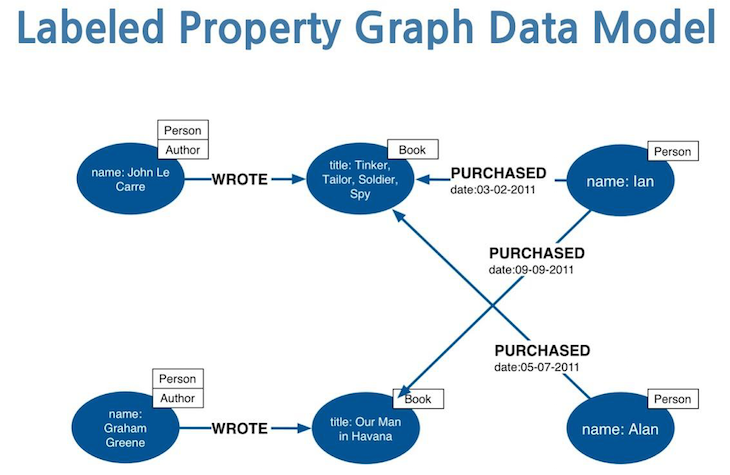
\includegraphics[width=0.75\textwidth]{neo4j}
\caption{The Neo4j model}
\label{fig:neo4j}
\end{figure}

Besides the aforementioned useful properties of Neo4j, we can put the graph to good use for visualising the global urban network. By adding a location property to a city, we can directly map nodes and relations to a geographical map. Most importantly, we can store indices of text files that mention the city as properties of nodes. That way, we are able to generate a subset of files that we can analyse for calculating the strength of the relationship between the nodes.









% --------------------------------------------Maybe useful in future----------------------------------------------------
\begin{comment}
\subsubsection{Elasticsearch}
Elasticsearch is an open-source search engine which centrally stores your data \cite{Elasticsearch}. It is a fast and scalable solution that was designed with big data search in mind. According to Kononenko et al. \cite{Kononenko2014} Elasticsearch has some significant advantages in comparison with traditional relational databases. Two of these advantages are scalability and performance. 

\paragraph{Scalability} According to Elasticsearch \cite{Elasticsearch} their product has no problem with scaling horizontally. It automatically manages indices and queries distributed across a cluster. This is an important feature as it is likely that the amount of data that our solution will use and process will increase and we do not want to keep upgrading the server that contains database, which would be vertical scalability. {\color{red} FIXME: Referentie naar dat we alleen NL doen nu? En daarom scalability nogal belangrijk is}

\paragraph{Performance}
Because Elasticsearch was designed to handle documents and perform full-text search it not surprising it performs well doing this. As we're going to be using the same kind of input data we expect Elasticsearch as the most choice. Kononenko et al. found that while scalability and schema-free documents are common for NoSQL systems, the combination of all three (scalability, agility, and performance) in one system is what makes Elasticsearch stand out from other systems. Following this, we conclude Elasticsearch would be a good choice as a data storage and search platform for our {\color{red} FIXME: solution|product|project.. (We moeten even kiezen welke we aanhouden zodat we dat overal hetzelfde doen}.\\

\paragraph{Downsides} \label{sec:elastic-downsides}
A downside of Elasticsearch is that it does not have any form of security out of the box. This means that everyone with the server address could access the data. This is not a problem for CommonCrawl data, as this was already available online anyway. However, when using for example Delpher or other sources you need a license this becomes a problem. Next to that, it would also be possible for anyone to meddle with the data in Elasticsearch making the data unreliable. Elasticsearch provides a Security package for which you unfortunately need a paid license. However, to secure Elasticsearch while making it available for users we could use a plugin such as Search Guard\footnote{\url{http://floragunn.com/searchguard/}} or use a special proxy as proposed by Kononenko et al. \cite{Kononenko2014}.

Another downside of Elasticsearch is that transactions involving multiple documents\footnote{\url{https://www.elastic.co/guide/en/elasticsearch/guide/current/concurrency-solutions.html}} are not ACIDic. Where ACID stands for the four properties atomicity, consistency, isolation and durability regarding transactions in database systems \cite{haerder1983principles}. This means that we need to keep concurrency problems in mind and will probably need to enable some locking to prevent these concurrency problems when performing transactions on multiple documents. 



\subsubsection{Hadoop}
Because we are designing a \maybe{application} that will use and parse a lot of data, it will be useful to use distributed computing. Although we only use the .nl data \maybe{Totale grootte van data noemen?} from CommonCrawl for this \todo{project} (see section \ref{sec:commoncrawl}) we could still benefit from distributed computing, especially with the future of the \maybe{application} in mind. 
Therefore we want to use Apache Hadoop, which is a framework that allows for the distributed processing of large data sets across clusters of computers using simple programming models \cite{Hadoop}. With this open source software we could distribute the computations from a single server across many more devices, thereby speeding up the process. 

\end{comment}
\subsection{Interacting with the Data}

For the application to be a success the processed data should be easily available to the end user. The data should be easy to query and should be presented in an accessible way.
We researched several options to offer the end user this experience.

\subsubsection{Query language}

The first option was to develop an easy to use/learn query language specific to our domain (intercity relations). For this we designed a simple query language with the following syntax.

\begin{center}
\begin{tabular}{ |c|c| } 
 \hline
 ! & Logic NOT operation \\
 \&\& & Logic AND operation \\ 
 $\|$ & Logic OR operation \\ 
 $( A \&\& B )$ & Grouping of clauses \\
 $A > R > B$ & Relation R between cities A and B \\
 \hline
\end{tabular}
\end{center}

Below, in figure \ref{fig:ql-example}, an example is shown that queries the "Shopping" relation between Rotterdam and Amsterdam and the same relation between Rotterdam and Den Haag.

\begin{figure}[ht]
\centering
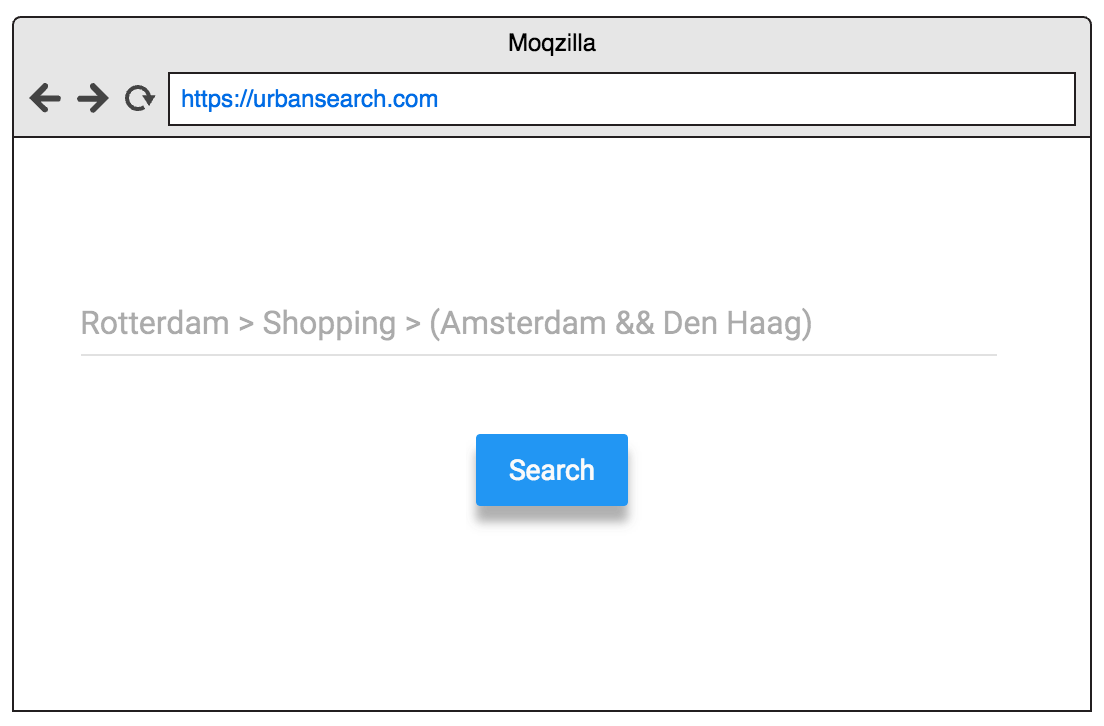
\includegraphics[width=0.75\textwidth]{ql-example}
\caption{Example interface for the query language}
\label{fig:ql-example}
\end{figure}

\subsubsection{Query composer interface}

Another option was to offer the end user a "query composition interface". This interface would have the same possibilities as the former mentioned query language, but should be more intuitive to use for new users. An example of the interface is given in figure \ref{fig:qi-example}.

\begin{figure}[ht]
\centering
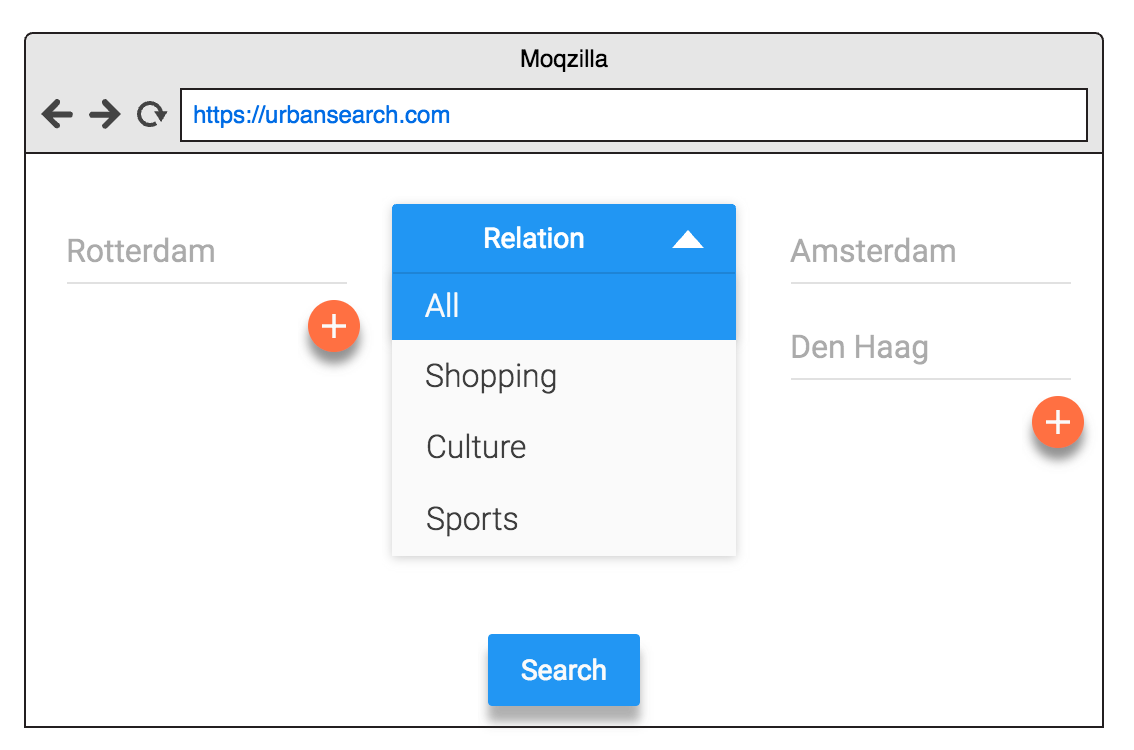
\includegraphics[width=0.75\textwidth]{qi-example}
\caption{Example of a query composer interface}
\label{fig:qi-example}
\end{figure}

\subsubsection{Interactive search}

The last option we investigated was an interactive approach to querying data. This means that the user interacts with a map containing relations and cities. A very simple example is given in figure \ref{fig:ii-example}.


\begin{figure}[ht]
\centering
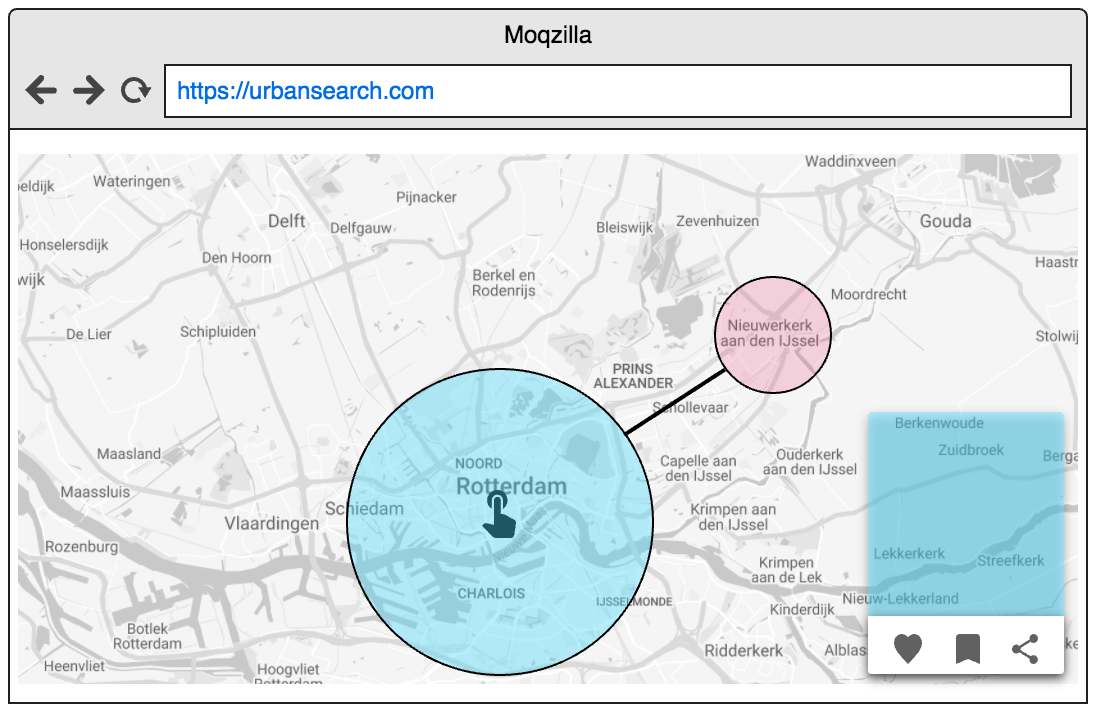
\includegraphics[width=0.75\textwidth]{ii-example}
\caption{Example of an interactive map}
\label{fig:ii-example}
\end{figure}

In this setup the user can click on cities and relations on the map which then triggers a query on the Neo4j back-end. The results can be visualised on the map (eg. showing information about the selected city).

\subsubsection{Conclusion}

Together with the client we decided that the best option was to go with the interactive map. This would lead to easy access to the data by the client and would fit better with the flow of use the client envisioned prior to the project. 
Also from the point of view of the researcher using the application, it fits a lot better in his/her work flow. The application is used to analyse and visualise relations between cities, if this can be done directly on the map it speeds up the users use of the system, since it is faster to select cities and relations on the fly. This helps make the application more intuitive since the user is probably more familiar with a map than with a new query language.
The creation of complex queries is also made a lot easier. The user doesn't have to write or compose a complex query in advance but can do it directly on the map. So getting a visual representation of several cities, interconnected with multiple relations, doesn't mean writing or composing a very long query but clicking/selecting cities and relations on the map.
Interaction directly with the map also reduces the need to go to a separate page to enter/compose a query. This speeds up the use of the system by reducing page loads and it interrupts the work flow of the user less.
A final advantage of using an interactive map over raw queries/query composition is that we don't have users entering invalid queries, this leads to less frustration using the system.
\subsection{Visualising the Data}

This section focuses on the visual representation of the processed data. Our goals are to present the data and the things we learned during the processing of the data in a way that is easy to comprehend for users and can help ease the interpretation of the data.
To reach these goals we focused on the clients needs and desires. We discussed the preferences off the client and drew up a global plan, which we present below.

\subsubsection{Representing the data visually}

Since we are dealing with strongly related data, which is comprised off cities and the relations between cities, it was a natural choice to represent the data as a graph.
The choice was made, together with the client, to show the nodes and relations on a map. This was done because people are used to cities being visualised on a map and we think this will increase the ability of users to interpret the information in a productive manner.

\subsubsection{Maps}

We investigated two technologies we could use for the map on which we will display our data. The first one is Google Maps (GM). GM can be used freely and offers a lot of customisation options. The API is well defined and some of the group members worked with GM before. The second option we investigated was Leaflet. Leaflet is an open-source javascript library which provides responsive maps. It also has an well defined API and a lot of plugins.
Both libraries are well suited for our needs. 
We decided to go with GM, because of the experience of the group members with using GM. Also we feel that there are more resources available on GM, which would help us if we get stuck with an issue.

\subsubsection{Map clutter}

One of the challenges of visualising networks, as stated in \cite{468391}, is the risk of so called map clutter. This means the network is displayed as an incomprehensible set of lines and nodes.
Several methods to prevent this are given in \cite{468391}. We will adopt some of these methods in our application. The methods and use of these methods in our application are presented next.
Users should be able to select what information they want to display. This will be adopted in our application by allowing the user to (de)select cities and relations, which then will be shown/hidden. The use of different sizes for nodes and edges or other attributes that are displayed can convey extra information to the user. We will use this to represent sizes of cities (population) and strengths of relations.
The use of colour is another method which is presented in \cite{468391}. We will use colours to represent different types of relations and we will use intensity/opacity to represent the strengths of these different types of relations.